% !TEX root = lfgw.tex
\chapter{Textpassagen in nicht-lateinischen Alphabeten einbetten}
%% \dictum[Donald E.\ Knuth, Professor Emeritus of The Art
%%   of Computer Programming, Stanford University]%
\dictum[Donald E.\ Knuth]%
{Hardcopy versions of the Unicode Standard have been among the
most crucial and most-heavily used reference books in my
personal library for years. Unicode allows me to celebrate the
fact that computer science is a vast worldwide
collaboration. And Unicode is perhaps the best tool I know to
help bring understanding between people of different
cultures.}

Hinweis von Lukas C. Bossert:
Für einzelne Wörter kann man auch \url{http://www.perseus.tufts.edu/hopper/morph} nutzen.
bzw. für antike Texte auch hieraus (\url{http://www.perseus.tufts.edu/hopper/collection?collection=Perseus:collection:Greco-Roman}) kopieren.

\section{Unicode}
\autor{Axel Kielhorn}\footcite{kielhorn:dtk2014}


\noindent Es war einmal \dots

Als \TeX{} in den 70er Jahren entwickelt wurde, war die Kodierung nach 
ASCII\footnote{Altertümlicher Standard Code Inzwischen Irrelevant} \emph{eine}
gängige Form Texte im Computer einzugeben. 
Die ersten 32 Zeichen waren Steuerzeichen, so blieben weniger als 100 druckbare Buchstaben.
Da dieser Standard aus den USA kam, gab es keine Umlaute oder sonstige europäische
Sonderzeichen.

Mit dem Erscheinen von \TeX{} 3.0 konnte \TeX{} auch 8-bit Kodierungen verarbeiten.
Ja, Kodierungen in der Mehrzahl, inzwischen hatten alle Computerhersteller den Zeichensatz
auf 8 bit erweitert, jeder nach seiner Art. Außerdem wurden in Mitteleuropa andere Buchstaben
benötigt als in Westeuropa.

\begin{labeling}{Mitteleuropa}
    \item[Westeuropa:]
      \emph{ISO-latin-1}, \emph{macroman}, \emph{hproman8}, \emph{CP850} und \emph{CP1252}
    \item[Mitteleuropa:]
      \emph{ISO-latin-2}, \emph{macromanCE}, \emph{CP852} und \emph{CP1250}
\end{labeling}

Je nach verwendetem System musste man auf einige Zeichen verzichten:

\begin{tabular}{lccccc}
    Latin-1		& «» 	& 		&	&	&	\\
    Latin-9		& «» 	&		& œ\,Œ	& €	&	\\
    CP1252		& «» 	& „“”	& œ\,Œ	& €	&	\\
    macroman	& «» 	& „“”	& œ\,Œ	& €(¤)	& fi\,fl	\\
    hproman		& «» 	& 		&	&	&	\\
\end{tabular}

Noch heute ist es bei einigen Betriebssystemen schwierig einige dieser 
\emph{exotischen} Zeichen direkt über die Tastatur einzugeben.

Bereits Anfang der 90er wurde eine Universelle Kodierung definiert,
die alle wichtigen Zeichen abdecken sollte.

Unicode wurde als 16-bit Kodierung entworfen, aber sehr schnell hat man festgestellt,
das 65tausend Zeichen nicht ausreichen und so wurde der Standard 1996
erweitert und umfasst jetzt 17 Ebenen (Planes) mit jeweils 65tausend
Zeichen. Somit ist es möglich auch Zeichen älterer Schriftsysteme
(Hieroglyphen, mittelalterliche Texte) und Fantasieschriften (Klingonisch,
Tengwar) in Unicode darzustellen.

Mit UTF-8 wurde eine platzsparende Kodierung entwickelt, die bei lateinischen Buchstaben
nur minimal mehr Platz benötigt als die alten 8-bit Systeme.

UFT-8 erfordert nicht zwingend ein unicodefähiges \TeX{}, solange man sich auf
lateinische Buchstaben beschränkt, funktioniert es auch mit \pdfTeX{}.

Heutzutage können alle Editoren mit Unicode umgehen, in Verbindung mit einem geeigneten
Zeichensatz lassen sich Zeichen wie {\FSEfont asdf άβγδἔ БГДЙ अऐक אשב ܚܤܜܗ} direkt eingeben.%
\footnote{Der in diesem Buch verwendetet Zeichensatz enthält nicht alle hier dargestellten Buchstaben.
Das Beispiel wurde daher in GNU FreeSerif \url{http://savannah.gnu.org/projects/freefont/} gesetzt.}

\section{Babel und Polyglossia}

Es gibt zwei Pakete, die sich um sprachspezifische Besonderheiten kümmern.
Außerdem gibt es noch den \paket{german.sty}, der spezielle Anpassungen für deutsche Texte
zur Verfügung stellt. Er sollte für neue Texte nicht mehr verwendet werden.

Das Paket \paket{babel} ist die international Weiterentwicklung des \paket{german.sty}.
Es bietet Unterstützung für mehr als 40 Sprachen und Dialekte und definiert neben den Trennmustern 
auch sprachabhängige Texte für das Datum (\cs{today}) sowie Überschriften für die Verzeichnisse 
(Inhaltsverzeichnis, Abbildungsverzeichnis, Literaturverzeichnis etc.).

<<<<<<< HEAD
Lange Zeit sah es so aus, als würde \paket{babel} nicht mehr weiterentwickelt.
=======
\begin{lfgwcode}{label={babel-preamble}}
 \documentclass{scrartcl}
 \usepackage[utf8]{inputenc} % nur bei pdflatex
 \usepackage[main=german,french]{babel}

 \begin{document}
 Text in Deutsch.
 Heute ist der \today.
 
 \begin{otherlanguage}{french}
 Aujourd'hui ce le \today.
 Ceci est en française!
 \end{otherlanguage}
 
 Und jetzt wieder ein Text in Deutsch!
 
 Beachte den Abstand vor dem Ausrufezeichen.
 Wörter oder kurze Sätze, 
 wie \foreignlanguage{french}{résistance} oder \foreignlanguage{french}{courant}
 werden nach den Regeln der Fremdsprache getrennt.
 
 Ganz schön spannend.
 
 \end{document}
\end{lfgwcode}

\begin{lfgwprint}{}
 Text in Deutsch.
 Heute ist der \today.
 
 \begin{otherlanguage}{french}
 Aujourd'hui ce le \today.
 Ceci est en française!
 \end{otherlanguage}
 
 Und jetzt wieder ein Text in Deutsch!
 
 Beachte den Abstand vor dem Ausrufezeichen.
 Wörter oder kurze Sätze, 
 wie \foreignlanguage{french}{résistance} oder \foreignlanguage{french}{courant}
 werden nach den Regeln der Fremdsprache getrennt.
 
 Ganz schön spannend.
\end{lfgwprint}

Im Beispiel \ref{babel-preamble} wird \paket{Babel} mit zwei Sprachen benutzt.
Die Hauptsprache wird mit der Option \texttt{main=} festgelegt.
Ohne diese Option ist die \emph{letzte} angegebene Sprache die Hauptsprache.
Im französischen Text wird ein kleiner Abstand vor dem \enquote{!} eingefügt.
Das passiert dank \paket{Babel} automatisch.

Fremdwörter werden am Zeilenende nach den Regeln der Fremdsprache getrennt,
wenn man sie entsprechend markiert.

Lange Zeit sah es so aus, als würde Babel nicht mehr weiterentwickelt.

In dieser Zeit entstand \paket{polyglossia} (Πολυγλωσσια), um die unicodefähigen \TeX{}-Versionen zu unterstützen.
Polyglossia bietet zusätzlich Unterstützung für Arabisch, Bengalisch, Farsi (Persisch), Hindi, Kannada, Khmer,
Koreanisch, Sanskrit, Syrisch, Tamil, Telugu, Thailändisch, Tibetisch und Urdu.
Für einige dieser Sprachen werden Funktionen benötigt, die in \LuaLaTeX{} nicht vorhanden sind.
Hier wird das Programm \XeLaTeX{} benötigt, das spezielle Unterstützung für Sprachen bietet,
die von Rechts nach Links geschrieben werden. Abgesehen davon gilt alles in diesem Buch über
\LuaLaTeX{} gesagte auch für \XeLaTeX{}.

Das Beispiel \ref{polyglossia-preamble} zeigt den Aufruf von \paket{Polyglossia}.
Obwohl Polyglossia eigene Befehle für die Sprachumschaltung verwendet, 
funktionieren die Babel Befehle weiterhin.

In der aktuellen Version (März 2017) hat \paket{Polyglossia} einen Fehler in Verbindung mit \LuaLaTeX{}.
Wenn einmal auf französische Zeichensetzung umgeschaltet wurde, bleibt das für den Rest des Dokumentes bestehen.

Seit Herbst 2013 bietet Babel Unterstützung für die Unicode basierten Engines.
Abhängig von der verwendeten Sprache kann entweder das eine oder as andere System besser sein.

Da sich beide Systeme weiterentwickeln ist dies für den konkreten Einsatzfall zu prüfen.

\begin{lfgwcode}{label={polyglossia-preamble}}
 \documentclass{scrartcl}
  \usepackage{polyglossia}
  \setmainlanguage[%
  	spelling=new,%old
  	latesthyphen=true,%false
	babelshorthands=true,%false
	]{german}
 \setotherlanguage{french}	
	
 \begin{document}
 Text in Deutsch.
 Heute ist der \today.

 \begin{french}
 Aujourd'hui ce le \today.
 Ceci est en française!
 \end{french}
 
 Und wieder in Deutsch!
 Beachte das Ausrufezeichen.
 Einzelne Wörter oder kurze Sätze, 
 wie \textfrench{résistance} oder \textfrench{courant}
 werden nach den Regeln der Fremdsprache getrennt.
 
 Ganz schön spannend.
 
 \end{document}
\end{lfgwcode}


\section{Eingabe von Unicode-Sonderzeichen}
\label{unicodeeingabe}\index{Unicode}

% Die Unicode Codepoint 2021 ist: Double Dagger, und sieht so aus: ``‡''
% Die Unicode Codepoint 2022 ist: Bullet, und sieht so aus: ``•''
% Die Unicode Codepoint 2045 ist: Left Square Bracket With Quill, und sieht so aus: ``⁅''
% Die Unicode Codepoint 2046 ist: Right Square Bracket With Quill, und sieht so aus: ``⁆''
% Die Unicode Codepoint 2e3f ist: Capitulum, und sieht so aus: ``⸿''
% Die Unicode Codepoint 02ad ist: Latin Letter Bidental Percussive, und sieht so aus: ``ʭ''
% Die Unicode Codepoint 169b ist: Ogham Feather Mark, und sieht so aus: ``᚛''
% Die Unicode Codepoint 169c ist: Ogham Reversed Feather Mark, und sieht so aus: ``᚜''
%
\subsection{Eingabe von Unicode-Zeichen in
einem \Program{Emacs} Buffer}
\label{unicodeviaemacs}\index{Unicode und Emacs}
\autor{Craig Parker-Feldmann}

Zwei Methoden ermöglichen die Eingabe von
Unicode-Zeichen in \Program{Emacs}:

\subsubsection*{Methode 1:\enspace Hexadezimalzahl eingeben}
\Program{Emacs}-Dokumentation benutzt die Schreibweise: %
\texttt{C-x 8}
um den Vorgang zu beschreiben: man druckt die Tastenkombination
\texttt{Strg}$+$\texttt{X} und dann \texttt{8}.
%% um den Vorgang zu beschreiben: man druckt die Tastenkombination
%% \Ctrl$+$\keystroke{X}\keystroke{8}.

In diesem Fall heisst das: %
\texttt{C-x 8}\meta{Eingabe}\meta{Unicode Codepoint}\meta{Eingabe}
ermöglicht die direkte Eingabe einer Unicode Zeichen.
%% In diesem Fall heisst das: %
%% \Ctrl$+$\keystroke{X}\keystroke{8}%
%% \Return{}%
%% \meta{Unicode Codepoint}%
%% \Return{} ermöglicht die direkte Eingabe einer
%% Unicode Zeichen.

Um einem \enquote{Capitulum} einzugeben: %
\texttt{C-x 8}\meta{Eingabe}\texttt{2e3f}\meta{Eingabe}
%% Um einem \enquote{Capitulum} einzugeben: %
%% \hbox{\Ctrl$+$\keystroke{X}}%
%% \keystroke{8}%
%% \Return{}%
%% \keystroke{2}\keystroke{E}\keystroke{3}\keystroke{F}%
%% \Return{}%
.

\subsubsection*{Methode 2:\enspace \Program{Emacs}-Aliase Benutzen}
\Program{Emacs} hat eine lange Liste vorgefertigte Aliase%
\footnote{Ein \enquote{Alias} ist eine Aufruf, mit der
mehrere Funktionen, durch einen neuen Befehl ersetzt werden kann.
Es wird benutzt, um Zeit zu sparen und weniger zu tippen.}%
um oft benutzte Unicode Zeichen einzugeben. Zuerst, mit nur
drei Tastendrücke: um eine \enquote{no-break space} einzugeben: %
\texttt{C-x 8}\meta{Leertaste}
%% \hbox{\Ctrl$+$\keystroke{X}}%
%% \keystroke{8}%
%% \Spacebar
.

Einige Aliase sind erst nach drei Tastendrücke fertig. Andere
benötigen vier Tastendrücke. Ich möchte das Wort \enquote{Français}
eingeben. Mit %
\texttt{C-x 8}\texttt{,c}
%% \hbox{\Ctrl$+$\keystroke{X}}%
%% \keystroke{,}%
%% \keystroke{c} %
kann ich einen \enquote{c} mit eine Cedille eingeben.

Ich möchte das Wort \enquote{mañana} eingeben. Mit %
\texttt{C-x 8}\texttt{\char126n}
%% \hbox{\Ctrl$+$\keystroke{X}}%
%% \keystroke{\char126}%
%% \keystroke{N} %
kann ich einen \enquote{n} mit einen Tilde eingeben.

Es gibt auch Aliase für drei verschiedene Bruchzahlen. Aber
\TeX{}-Benutzer haben nie Probleme damit gehabt, Bruchzahlen
zu setzen.

%% \subsection{Eingabe von Unicode-Zeichen in Linux-GNOME Programme}
%% \label{unicodeviagnome}
%% Einige Anwendungen in den Linux GNOME-Oberfläche
%% (z.\,B.\ \Program{gnome-terminal} und \Program{gedit})
%% ermöglichen die direkt Eingabe von Unicode Zeichen durch
%% Tastendruck-Folge %
%% \hbox{\Shift$+$\Ctrl$+$\keystroke{U}}%
%% \meta{Unicode Codepoint}%
%% \Return{}.

%% Mit %
%% \hbox{\Shift$+$\Ctrl$+$\keystroke{U}}%
%% \keystroke{2}\keystroke{0}\keystroke{2}\keystroke{2}%
%% \Return{} %
%% kann ich einen \enquote{Bullet} eingeben.

\minisec{Eingabe direkt mit der Tastatur}

Lohnend besonders bei den modernen Fremdsprachen: Anschaffen einer Tastatur in der jeweiligen
Sprache.

Dabei muss es sich nicht um eine physikalische Tastatur handeln.
Oft reicht es, die entsprechende Tastatur im Betriebssystem zu aktivieren und sich das
Tastaturlayout auszudrucken.
So kann man die Zeichen direkt eingeben, auch wenn auf den Tasten etwas anderes steht.
Alternativ kann man eine Bildschirmtastatur benutzen.

Problem im altphilologischen Bereich: Akzente und (bei Hebräisch) Vokalzeichen sind heute
nicht mehr verwendet und fehlen deshalb auf den heutigen Tastaturen.

\minisec{Auswahl über Maus-gestützte tools}
KCharselect

\begin{figure}
 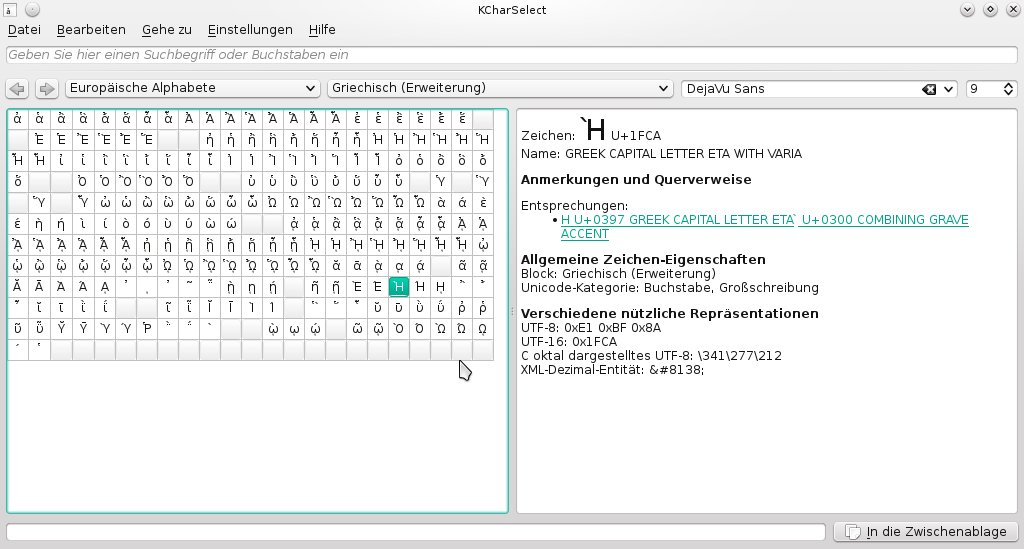
\includegraphics[width=\textwidth]{kcharselect}
 \caption{Mit dem KDE-Programm KCharselect kann man Unicode-Buchstaben immerhin mit der Maus
 auswählen.}
\end{figure}

\minisec{Eingabe über die Zeichennummer}

Vgl.\ Abschnitt \ref{utf8codes} auf Seite \pageref{utf8codes}.

\section{Griechisch}
\index{Griechisch}

Es gibt (mindestens...) drei verschiedene Möglichkeiten, griechische Textpassagen einzubinden;
je nach Aufgabenberich sind diese verschieden gut geeignet:


\minisec{Möglichkeit I: Einzelbuchstaben}

Die erste Möglichkeit besteht in der Eingabe m.\,H. der Einzelbuchstaben-Symbole des Paketes
\paket{textgreek}; das Verfahren ist in  \fullref{griechEinzelbuchstaben} beschrieben.

Dieses Verfahren eignet sich eigentlich nur für ganz kurze Einsprengsel im Umfang von
einzelnen Zeichen bis maximal ca.\ einem Wort.


\minisec{Möglichkeit II: Transkription mit \paket{ibycus}}

Die zweite Methode eignet sich demgegenüber hervorragend, wenn es darum geht auch etwas
längere (alt-)griechische Passagen in ein ansonsten deutschsprachiges Dokument~-- m.\,H. eines
deutschen Computers mit QWERTZ-Tastatur~-- einzugeben.

Dabei wird für die griechischen Buchstaben eine Art Transkription in lateinischen Buchstaben
vorgenommen, die sich bei etwas Übung sehr leicht benutzen lässt.

Das Paket \paket{ibycus}%
\footnote{Paketdokumentation: \file{texdoc ibycus-babel}}
definiert dabei eine Art Pseudosprache für \paket{babel},
in der Dokumenpräambel ist also anzugeben:

\begin{lstlisting}
 \usepackage[ibycus,ngerman]{babel}
\end{lstlisting}

Im Dokument stehen dann eine Umgebung \env{ibycus} sowie ein Befehl \cs{ibygr\{\}}
zur Verfügung:


Das wird zu:

 \begin{ibycus}
  (Hrodo'tou Qouri’ou i(stori’hs a)po’decis h(’de,
  ...
  h(‘n ai)ti’hn e)pole’mhsan a)llh’loisi.
  \end{ibycus}

  Und jetzt ein einzelnes griechisches Wort~-- \ibygr{a)rxai=a gra’mmata}~-- im Text.





\minisec{Möglichkeit III: Direkteingabe von Unicode-Text}

Die dritte Möglichkeit besteht darin, die griechischen Schriftzeichen direkt als Unicode-Zeichen
in das \LaTeX -Dokument einzufügen. Dazu reicht es aus, dem Paket \paket{babel} die
(alt"~)""griechische Sprache als zusätzliche Option anzugeben:
\cs{usepackage\oarg*{polutonikogreek,ngerman}\marg*{babel}}.
\footnote{Achtung! Bei den meisten \LaTeX-Installationen im Rahmen von Linux-Distributionen muss
man Pakete nachinstallieren!}
Damit \LaTeX{} den griechischen Font richtig ansprechen kann, braucht auch das Paket \paket{fontenc}
eine Modifikation: \cs{usepackage\oarg*{OT1,T1}\marg*{fontenc}}.

Dann kann mit \cs{selectlanguage\marg*{polutonikogreek}} auf Griechisch umgeschaltet werden.

Der folgende Bibelvers wurde aus dem Internet unverändert in das \LaTeX-Dokument
kopiert. Derzeit werden nicht alle Zeichen in meinem KDE-Editor (kile) korrekt dargestellt (vgl. Abb.);
dennoch gibt \LaTeX{} alle Zeichen richtig wider:

\begin{figure}
 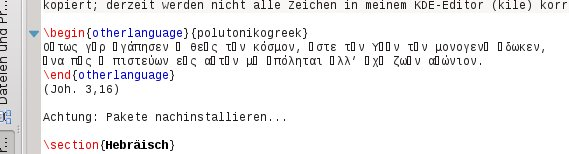
\includegraphics[width=\textwidth]{ersatzdarstellung}
 \caption{KDE kann nicht alle aus dem Internet kopierten Unicode-Zeichen korrekt darstellen;
 Buchstaben mit Akzent und Spiritus bekommen eine (nichtssagende) Ersatzdarstellung!}
\end{figure}


\begin{otherlanguage}{polutonikogreek}
Οὕτως γὰρ ἠγάπησεν ὁ Θεὸς τὸν κόσμον, ὥστε τὸν Υἱὸν τὸν μονογενῆ ἔδωκεν,
ἵνα πᾶς ὁ πιστεύων εἰς αὐτὸν μὴ ἀπόληται ἀλλ’ ἔχῃ ζωὴν αἰώνιον.
\end{otherlanguage}
(Joh. 3,16)

Diese Methode dürfte sich in der Praxis am ehesten eignen, wenn bereits ein Textcorpus
(z.\,B. via Internet) ediert und Unicode-Erfasst vorliegt, und Textpartien ins eigene Dokument
ohne Veränderungen übernommen werden sollen~-- so wie z.\,B. bei Zitaten aus der Bibel oder
der klassischen Literatur.

Will man selbst (alt"~)""griechische Textpassagen schreiben, scheint das Ibykus-Verfahren
wesentlich angenehmer und effizienter.


\section{Hebräisch}
\index{Hebräisch}

Das Paket \paket{cjhebrew} von Christian Justen eignet sich hervorragend für
Theologen und Orientalisten, denn es erlaubt auch die Vokalisierung sowie die Verwendung
von Akzenten. Auch das Problem der rechts- bzw. linksläufigen Schriften wird sehr
Anwenderfreundlich~-- im Sinne von Anwendern an einem westlichen PC mit ansonsten
lateinischen Alphabet~-- gelöst:

Nach \cs{usepackage\marg*{cjhebrew}}%
\footnote{Eine besondere Angabe z.\,B. bei \paket{babel} ist nicht nötig.}
steht v.\,a. der Befehl \cs{cjRL\{\}}
-- für hebräische Einzelworte im laufenden Absatz~-- sowie die
Umgebung \lstinline/cjhebrew/
-- für ganze Absätze in Hebräisch~-- zur Verfügung.

Beide drehen die Folge der Schriftzeichen automatisch um, so dass hebräische Textpartien
ganz gewohnt eingegeben werden können. Dabei sind für die einzelnen Zeichen sehr leicht
merkbare Codes definiert worden:

Der Beginn des biblischen Buches Genesis~-- \enquote{Im Anfang schuf Gott Himmel und Erde\dots} --
wird so eingegeben:

\begin{lstlisting}
\begin{cjhebrew}
 b*e:re'+siyt b*ArA' 'E:lohim 'et ha+s*amayim w:'et hA'ArE.s;
\end{cjhebrew}
\end{lstlisting}

Mit etwas Eingewöhnung arbeitet man mit diesem System \emph{wesentlich} schneller und
angenehmer, als wenn man etwa die Unicode-Zeichen mit Hilfe eines grafischen Auswahlwerkzeuges
einzeln auswählt...

Die Bearbeitung mit \LaTeX{} ergibt:

\begin{cjhebrew}
 b*e:re'+siyt b*ArA' 'E:lohim 'et ha+s*amayim w:'et hA'ArE.s;
\end{cjhebrew}

Wegen der Einzelheiten der Zeichen-, Vokal-, Akzent- und Satzzeichen-Codierung (inkl. z.\,B.
Mem finalis) sei auf die Paketdokumentation verwiesen.

\section{Russisch}
\index{Kyrillisch}
\index{Russisch}

\section{Koptisch}
\index{Koptisch}

\section{Altkirchenslawisch}
\index{Altkirchenslawisch}

\paket{churchslavonic}


\section{Arabisch}
\index{Arabisch}

Ist \paket{arabtex} noch aktuell?
%Philipp sagt: ansonsten sah ich grad dies: http://www.ctan.org/pkg/arabluatex

\section{Hieroglyphen}
\index{Hieroglyphen}
\index{Ägyptologie}

\paket{hieroglf}~-- \enquote{The Poor Man’s Hieroglyphic Font}


 \pmglyph{K:l-i-o-p-a-d:r-a}


\section{Keilschrift}
\index{Keilschrift}

\paket{archaic} und andere...

\section{Runen}
\index{Runen}

Das Paket \paket{runic} von Peter Wilson stellt die Runen des sog.\ Futhark-Alphabets bereit.
Nach \lstinline/\usepackage{runic}/ gibt es den Befehl \lstinline/\textfut{}/, der
die Runen ausgibt. Dies ist die Transkription:

\begin{center}
\begin{tabular}{ll}
 \lstinline/F/ &	\textfut{F} \\
 \lstinline/U/ &	\textfut{U} \\
 \lstinline/\Fthorn/ &	\textfut{\Fthorn} \\
 \lstinline/A/ &	\textfut{A} \\
 \lstinline/R/ &	\textfut{R} \\
 \lstinline/K/ &	\textfut{K} \\
 \lstinline/G/ &	\textfut{G} \\
 \lstinline/W/ &	\textfut{W} \\
 \lstinline/H/ &	\textfut{H} \\
 \lstinline/N/ &	\textfut{N} \\
 \lstinline/I/ &	\textfut{I} \\
 \lstinline/J/ &	\textfut{J} \\
 \lstinline/Y/ &	\textfut{Y} \\
 \lstinline/P/ &	\textfut{P} \\
 \lstinline/X/ &	\textfut{X} \\
 \lstinline/S/ &	\textfut{S} \\
 \lstinline/T/ &	\textfut{T} \\
 \lstinline/B/ &	\textfut{B} \\
 \lstinline/E/ &	\textfut{E} \\
 \lstinline/M/ &	\textfut{M} \\
 \lstinline/L/ &	\textfut{L} \\
 \lstinline/\Fng/ &	\textfut{\Fng} \\
 \lstinline/D/ &	\textfut{D} \\
 \lstinline/O/ &	\textfut{O} \\
 \lstinline/:/ &	\textfut{:} \\
 \end{tabular}
 \end{center}


\section{Phonetische Alphabete}


\section{Kurzschriften}
\index{Kurzschrift}
\index{Schnellschrift}

\minisec{Tironische Noten}
\index{Tironische Noten}


\minisec{Deutsche Einheits-Kurzschrift}
DEK\footcite{sarman:dtk2009/1}
\index{Deutsche Einheits-Kurzschrift}
\index{DEK}


\minisec{Pitman-Kurzschrift}
\index{Pitman}
